\chapter{Aktywności}

Ten rozdział opisuje aktywności systemu. Są one rozszerzeniem opisów wymagań funkcjonalnych z analizy biznesowej \cite{dokumentacja}.

\section{Rozpoczęcie nowej gry}

Rysunek 6.1 przedstawia diagram aktywności rozpoczęcia nowej rozgrywki.
Na ekranie menu głównego gracz będzie mógł wybrać opcję nowej gry. Po jego wciś\-nię\-ciu aplikacja rozpocznie proces generowania części terenu, flory i fauny. Gdy obiekty zostaną wygenerowane, zostanie z nich utworzona plansza gry. Następnie zostanie zainicjalizowana postać gracza i wyświetlony zostanie widok rozgrywki.

\begin{figure}[H]
    \centering
        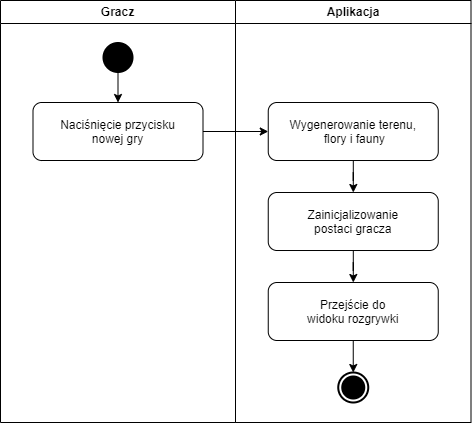
\includegraphics[width=0.7\textwidth]{Graphics/activities/new_game.png}
         \index{Diagram aktywności rozpoczęcia nowej gry}
         \caption{Diagram aktywności rozpoczęcia nowej gry}
\end{figure}

\clearpage

\section{Zapis rozgrywki}

Rysunek 6.2 przedstawia diagram aktywności zapisu rozgrywki.
Podczas rozgrywki gracz będzie mógł włączyć \textit{menu} i wybrać z niego opcję zapisu. Po wybraniu aplikacja wyświetli panel zapisu, z którego gracz będzie mógł wybrać pole zapisu i nacisnąć odpowiedni przycisk, by zapisać aktualny stan rozgrywki. Jeżeli pole było już zajęte, to gracz zostanie zapytany, czy chce nadpisać wskazany zapis. Jeżeli to zrobi, stan rozgrywki zapisze się. W przeciwnym wypadku rozgrywka nie zapisze się. Jeżeli pole było puste, to rozgrywka się zapisze.

\begin{figure}[H]
    \centering
        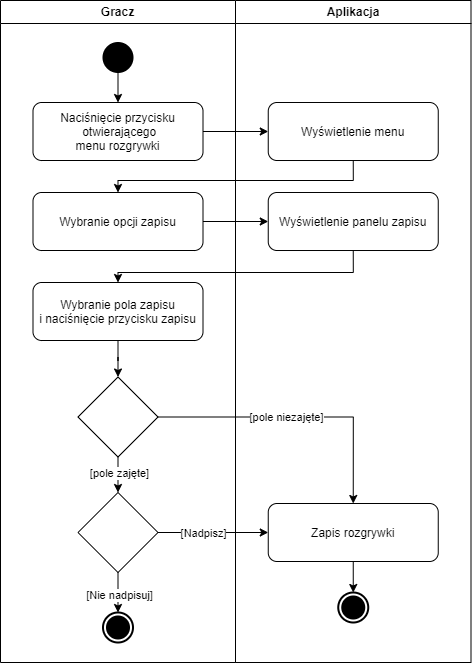
\includegraphics[width=0.7\textwidth]{Graphics/activities/save_game (1).png}
         \index{Diagram aktywności zapisu rozgrywki}
         \caption{Diagram aktywności zapisu rozgrywki}
\end{figure}

\clearpage

\section{Wczytanie rozgrywki}

Rysunek 6.3 przedstawia diagram aktywności wczytania rozgrywki.
Na ekranie menu głównego gracz będzie mógł wybrać opcję wczytania rozgrywki. Po wybraniu aplikacja otworzy panel wczytania rozgrywki. Gracz będzie mógł wybrać zapis który chce załadować i nacisnąć przycisk wczytaj, aby załadować stan wybranej rozgrywki. Po załadowaniu stanu rozgrywki wyświetlony zostanie widok rozgrywki.

\begin{figure}[H]
    \centering
        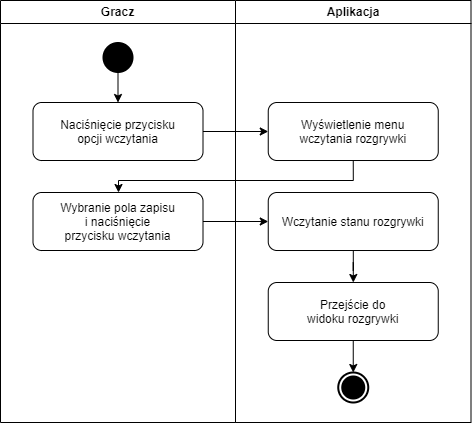
\includegraphics[width=0.7\textwidth]{Graphics/activities/load_game.png}
         \index{Diagram aktywności wczytania rozgrywki}
         \caption{Diagram aktywności wczytania rozgrywki}
\end{figure}

\clearpage

\section{Zmiana ustawień}

Rysunek 6.4 przedstawia diagram aktywności zmiany ustawień.
Na ekranie menu głównego gracz będzie mógł wybrać opcję zmiany ustawień. Po wybraniu aplikacja wyświetli menu zmiany ustawień. Po wybraniu ustawień gracz będzie mógł kliknąć przycisk zapisu ustawień. Jeżeli to zrobi aplikacja zapisze zmienione ustawienia.

\begin{figure}[H]
    \centering
        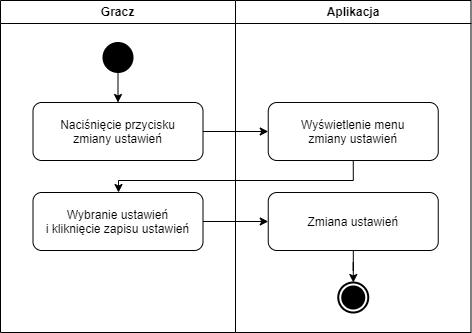
\includegraphics[width=0.7\textwidth]{Graphics/activities/change_options.png}
         \index{Diagram aktywności zmiany opcji}
         \caption{Diagram aktywności zmiany opcji}
\end{figure}

\clearpage

\section{Wyłączenie rozgrywki}

Rysunek 6.5 przedstawia diagram aktywności wyłączenia rozgrywki.
Podczas rozgrywki gracz będzie mógł wcisnąć przycisk \textit{menu}. Aplikacja wyświetli wówczas menu rozgrywki. Gracz będzie mógł wybrać opcję zakończenia rozgrywki. Aplikacja wyświetli możliwość zapisu rozgrywki przed zakończeniem. Jeżeli gracz wybierze opcje wyjścia bez zapisu, to rozgrywka zakończy się. Jeżeli gracz wybierze opcje zapisu przed zakończeniem, to otworzy się ekran zapisu. Gracz będzie mógł wybrać pole zapisu. Po zakończonym zapisie rozgrywka zakończy się.

\begin{figure}[H]
    \centering
        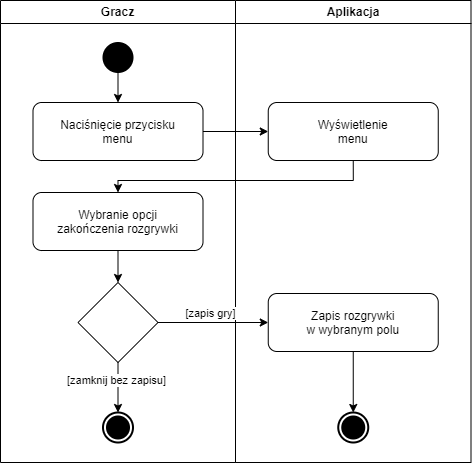
\includegraphics[width=0.7\textwidth]{Graphics/activities/exit_game.png}
         \index{Diagram aktywności wyłączenia rozgrywki}
         \caption{Diagram aktywności wyłączenia rozgrywki}
\end{figure}

\clearpage

\section{Użycie samouczka}

Rysunek 6.6 przedstawia diagram aktywności użycia samouczka.
Podczas rozgrywki gracz będzie mógł wcisnąć przycisk \textit{samouczka}. Po wciśnięciu gra wyświetli menu dialogowe, z którego użytkownik będzie mógł wybrać interesujące go zagadnienie. Po wyborze gra wyświetli opis danego zagadnienia.

\begin{figure}[H]
    \centering
        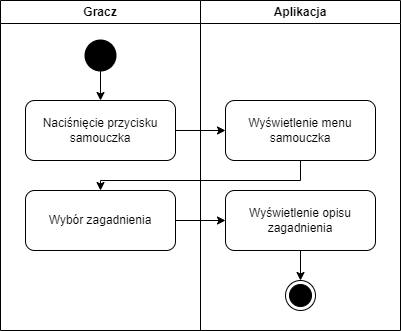
\includegraphics[width=0.7\textwidth]{Graphics/activities/tutorial.png}
         \index{Diagram aktywności użycia samouczka}
         \caption{Diagram aktywności użycia samouczka}
\end{figure}

\clearpage

\section{Poruszanie się}

Rysunek 6.7 przedstawia diagram aktywności poruszania się.
Podczas rozgrywki gracz będzie mógł nacisnąć przyciski \textit{ruchu}. Wciśnięcie któregoś rozpocznie ruch postaci. Postaci nadana zostanie prędkość o kierunku zależnym od kierunku kamery i wciśniętych przycisków. Postać będzie się przemieszczać tak długo, jak wciśnięty będzie przynajmniej jeden przycisk ruchu. Jeżeli gracz wciśnie w trakcie ruchu przycisk \textit{skoku} to postać przejdzie w stan skoku. Jeżeli po zakończeniu skoku dalej wciśnięte są przyciski \textit{ruchu}, to ruch będzie kontynuowany. W przeciwnym przypadku ruch zakończy się.

\begin{figure}[H]
    \centering
        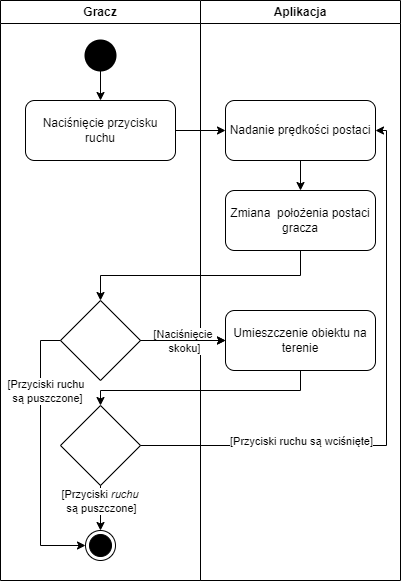
\includegraphics[width=0.7\textwidth]{Graphics/activities/move.png}
         \index{Diagram aktywności poruszania się}
         \caption{Diagram aktywności poruszania się}
\end{figure}

\clearpage

\section{Skanowanie}

Rysunek 6.8 przedstawia diagram aktywności skanowania.
Podczas rozgrywki gracz będzie mógł nacisnąć przycisk \textit{skanowania}. Jeżeli kamera będzie wycelowana w obiekt, który można zeskanować, to rozpocznie proces skanowania. Aplikacja wyświetli wówczas animacje skanowania. Po skończeniu animacji odpowiedni obiekt dodany zostanie do katalogu gracza. Jeżeli gracz trzyma dalej wciśnięty przycisk \textit{skanowania}, to aplikacja sprawdzi, czy obiekt można zeskanować. Jeżeli tak to powtórzy proces. Jeżeli nie będzie można zeskanować lub gracz puści przycisk to skanowanie zakończy się.

\begin{figure}[H]
    \centering
        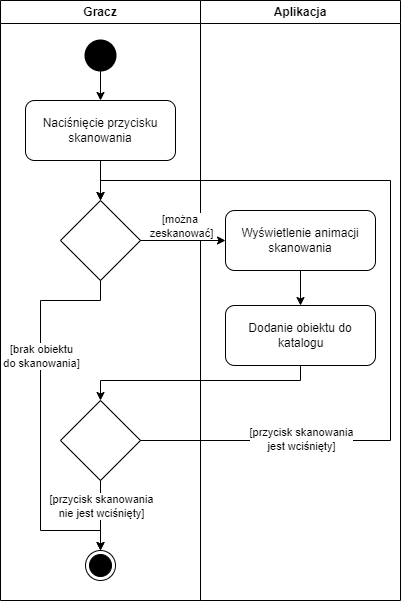
\includegraphics[width=0.7\textwidth]{Graphics/activities/scan.png}
         \index{Diagram aktywności skanowania}
         \caption{Diagram aktywności skanowania}
\end{figure}

\clearpage

\section{Jedzenie}

Rysunek 6.9 przedstawia diagram aktywności jedzenia.
Podczas rozgrywki gracz będzie mógł wykonać akcję jedzenia. Jeżeli wartość wskaźnika najedzenia postaci będzie maksymalna, to nie zje ona i aktywność się zakończy. Jeżeli wartość wskaźnika najedzenia nie będzie maksymalna to liczba jednostek posiadanego jedzenia danego typu zmniejszy się, a wskaźnik najedzenia zwiększy swoją wartość.

\begin{figure}[H]
    \centering
        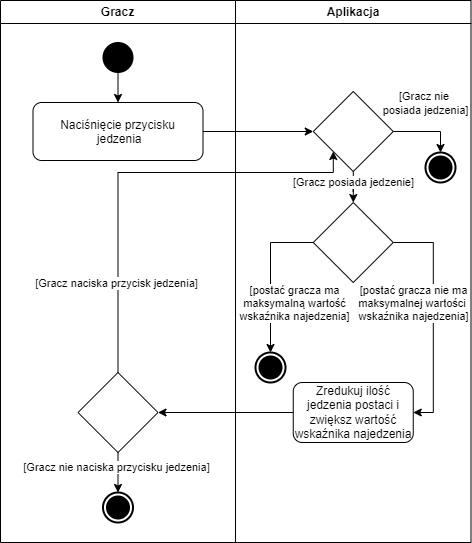
\includegraphics[width=0.7\textwidth]{Graphics/activities/eat.png}
         \index{Diagram aktywności jedzenia}
         \caption{Diagram aktywności jedzenia}
\end{figure}

\clearpage

\section{Budowanie}

Rysunek 6.10 przedstawia diagram aktywności budowania.
Podczas rozgrywki gracz będzie mógł włączyć \textit{menu budowania}. Po naciśnięciu odpowiedniego przycisku gra wyświetli menu budowania. Gracz będzie mógł wybrać jeden z obiektów do zbudowania. Jeżeli to zrobi oraz obiekt będzie mógł być postawiony, to zostanie on umieszczony w danej lokalizacji. Jeżeli nie będzie mógł być postawiony, to aplikacja wróci do menu wyboru budowli. Jeżeli gracz zdecyduje się nie stawiać budowli, to menu zamknie się.

\begin{figure}[H]
    \centering
        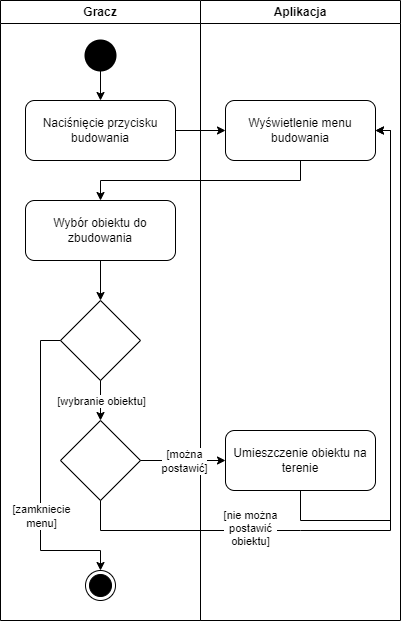
\includegraphics[width=0.7\textwidth]{Graphics/activities/build.png}
         \index{Diagram aktywności budowania}
         \caption{Diagram aktywności budowania}
\end{figure}

\clearpage

\section{Zbieranie surowców}

Rysunek 6.11 przedstawia diagram aktywności zbierania surowców.
Podczas rozgrywki gracz będzie mógł wcisnąć przycisk \textit{zbierania}. Jeżeli kamera będzie wycelowana w obiekt, z którego zebrać można surowce, to rozpocznie się proces zbierania. Aplikacja wyświetli wówczas animacje zbierania. Po skończeniu animacji odpowiedni surowiec dodany zostanie do ekwipunku gracza. Jeżeli gracz nadal trzymać będzie wciśnięty przycisk \textit{zbierania}, to aplikacja sprawdzi, czy z obiektu można zebrać surowce. Jeżeli tak to powtórzy proces. Jeżeli nie będzie można ich zebrać lub gracz puści przycisk, zbieranie zakończy się.

\begin{figure}[H]
    \centering
        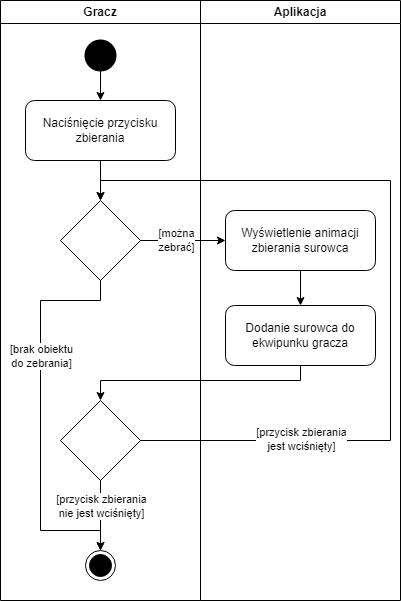
\includegraphics[width=0.7\textwidth]{Graphics/activities/gathering_materials.png}
         \index{Diagram aktywności zbierania surowców}
         \caption{Diagram aktywności zbierania surowców}
\end{figure}

\clearpage

\section{Zabijanie zwierząt}

Rysunek 6.12 przedstawia diagram aktywności zabijania zwierząt.
Podczas rozgrywki gracz będzie mógł wcisnąć przycisk \textit{zabijania}. Jeżeli kamera będzie wycelowana w żywe zwierze, to rozpocznie się proces zabijania. Aplikacja wyświetli wówczas animacje zabijania. Po skończeniu animacji, aplikacja zmniejszy wartość wskaźnika życia zwierzęcia i jeżeli wartość wskaźnika życia danego zwierzęcia wyniesie 0, to stan zwierzęcia zmieni się na zabity i proces zabijania się zakończy. Jeżeli wartość wskaźnika życia danego zwierzęcia będzie większa od 0, to aplikacja sprawdzi, czy przycisk \textit{zabijania} dalej jest wciśnięty. Jeżeli jest, to proces zabijania będzie kontynuowany. Jeżeli nie będzie można zabić zwierzęcia, zwierze będzie zabite lub gracz puści przycisk, zabijanie zakończy się.

\begin{figure}[H]
    \centering
        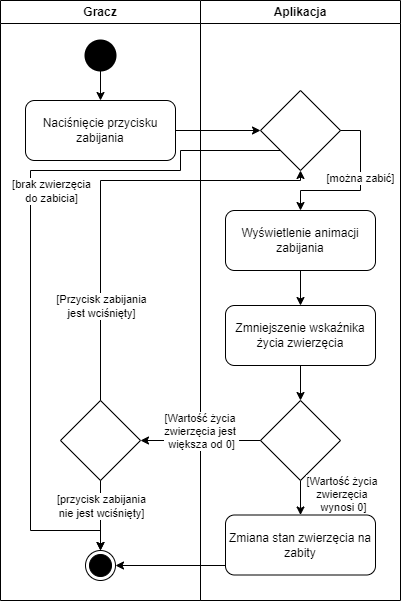
\includegraphics[width=0.65\textwidth]{Graphics/activities/killing_animal.png}
        \index{Diagram aktywności zabijania zwierząt}
        \caption{Diagram aktywności zabijania zwierząt}
\end{figure}